\begin{figure}[h]
  \centering
  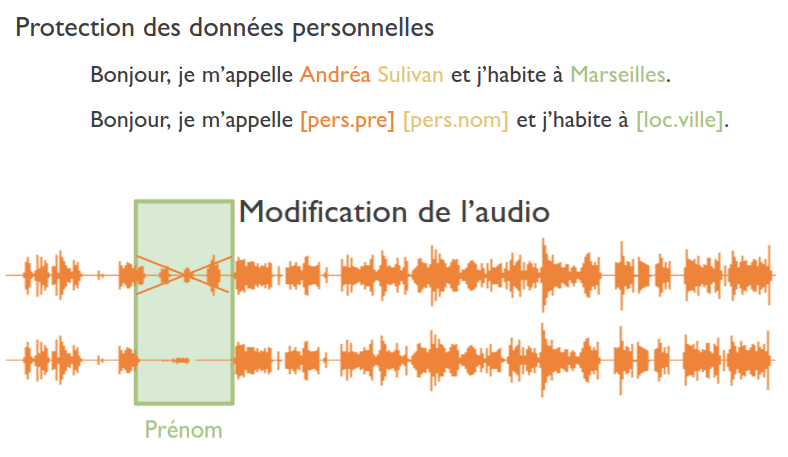
\includegraphics[width=15cm]{./Chapitre4/figures/annony.png}
  \caption{Exemple d'obfuscation d'un segment fictif. Les mots sont d'abord retrouvés dans la transcription, puis sont substitués par leur catégorie. Enfin le signal audio est modifié pour remplacer les informations personnelles par un son pré-enregistré.}
  \label{fig:annony}
\end{figure}
